% !TEX program = xelatex
\documentclass{diploma_style}

\def\b3d{B\textsuperscript{3}D}

\author{\href{mailto:balint.balazs@embl.de}{Bálint Balázs}}
\supervisor{\href{mailto:hufnagel@embl.de}{Lars Hufnagel}, \href{mailto:rozsabal@koki.hu}{Balázs Rózsa}}
\lab{\href{http://www.embl.de/}{European Molecular Biology Laboratory}}
\university{\href{http://www.ppke.hu/}{Pázmány Péter Catholic University}}
\collegeordept{\href{http://www.itk.ppke.hu/}{Faculty of Information Technology}}
\degreedate{A thesis submitted for the degree of \\ \textit{Doctor of Philosophy} \\ 2017}
\ppke{
\includegraphics[width=2cm]{figures/0_front/ITK_logo}}
\embl{
\includegraphics[width=5cm]{figures/0_front/EMBL_logo}}
\degree{PhD}

\title{Title goes here}
%\date{2012 november}
\begin{document}

\maketitle
\pagenumbering{roman}

%% spellcheck-language hu-HU
%\begin{nyilatkozat}
%Alulírott Balázs Bálint, a Pázmány Péter Katolikus Egyetem Információs Technológiai Karának hallgatója kijelentem, hogy ezt a szakdolgozatot meg nem engedett segítség nélkül, saját magam készítettem, és a szakdolgozatban csak a megadott forrásokat használtam fel. Minden olyan részt, melyet szó szerint, vagy azonos értelemben, de átfogalmazva más forrásból átvettem, egyértelműen a forrás megadásával megjelöltem. Ezt a Szakdolgozatot más szakon még nem nyújtottam be.

%% spellcheck-language en-US
%I, Balázs Bálint, student of Pázmány Péter Catholic University Faculty of Information Technology, herewith declare that I have produced this paper without the prohibited assistance of third parties and without making use of aids other than those specified; notions taken over directly or indirectly from other sources have been identified as such. This thesis has not previously been presented in identical or similar form to any other examination board.

%\vspace{1em}
%Budapest, 2013.05.16.

%\vspace{20mm}
%\hspace{90mm}
%signature
%aláírás
%\end{nyilatkozat}

%% spellcheck-language hu-HU
\begin{absztrakt}
Absztrakt magyarul.
\end{absztrakt}

%% spellcheck-language en-US
\begin{abstract}
Abstract in English.
\end{abstract}



\tableofcontents
\setcounter{page}{1}
\pagenumbering{arabic}

\chapter*{Introduction}
\addcontentsline{toc}{chapter}{Introduction}
\cite{huisken_optical_2004}




\chapter{Light-sheet microscopy}

Light microscopy is one of the oldest methods that is still widely used today to investigate the inner workings of microscopic life. Light-sheet microscopy is a relaviely new addition to the arsenal of tools that comprise light microscopy methods, and is especially suitable for live imaging of embryonic samples over extended periods of time \cite{krzic_multiview_2012,tomer_quantitative_2012}. It is also easily adapted to the sample, allowing to image a large variaty of specimens, from entire organs, such as cleared mouse brains \cite{dunsby_optically_2008}, to the subcellular processes occuring inside cultured cells \cite{capoulade_quantitative_2011}.

\section{Fluorescence microscopy}
Fluorescence microscopy \cite{lichtman_fluorescence_2005} 
 very small amount of illumination photons will result in fluorescence ($<0.0001\%$), the signal to noise ratio of the fluorescence is still very high due to the filtering.

good for live, naturally fluorescent structures

autofluorescence not specific
fluorescent dyes
fluorescent proteins
Nobel Prize in chemistry in 2008 GFP \cite{service_three_2008}
lot of fluorescent proteins since then \cite{shaner_guide_2005}. 
benefits: cell is producing
using genetic techniques possible to bind to other proteins, and specifically label structures of interest

\subsection{Wide-field fluorescence microscopy}
(Figure \ref{fig:wide-field})
regular microscope -> figure for this?
filter cube

\begin{figure}[htbp]
    \centering
    \includegraphics[page=4,scale=0.8]{figures/1_spim/spim_cyl}
    \caption{\textbf{Wide-field fluorescent microscope.}}
    \label{fig:wide-field}
\end{figure}

\subsubsection{Resolution of a wide-field microscope}

resolution
smallest distance of two points still distinguishable
few different definitions
this is because of diffraction
Airy pattern
Rayleigh criterion -> Abbe's formula
$d = 0.61 \frac{\lambda}{NA}$
plus axial resolution
$d_z = \frac{2\lambda}{NA^2}$

this result is base on the paraxial approximation of the Helmholtz equation, thus only apply for small NA.
a more general method to calculate resolution for high NA imaging systems is SGH:
A generally accepted method to calculate lateral ($\sigma_{xy}$) and axial ($\sigma_{z}$) resolution of an optical microscope is described by the Stelzer-Grill-Heisenberg, or SGH~theory\cite{grill_method_1999, stelzer_uncertainty_2000}:
A more general expression, works for large NA as well
\begin{equation} \label{eq:latres}
\sigma_{xy}=\frac{\lambda}{\sqrt{3-2 \cos \alpha - \cos 2 \alpha}}
\end{equation}
\begin{equation} \label{eq:axres}
\sigma_z = \frac{\lambda}{1-\cos \alpha}
\end{equation}
Generally, instead of $\alpha$, the numerical aperture (NA) is commonly used to characterize a lens' aperture. 
$NA=n\cdot \sin \alpha$, where n is the refractive index of the medium and $\alpha$ stands for the angular aperture.

even for high NA axial/lateral ratio $\sim 3-6$ (Figure~\ref{fig:resolution})
In principle it is possible to achieve isotropic resolution by increasing the acceptance angle to $\alpha = 180^\circ$, which means all light needs to be collected from the sample. Designing an objective that is capable of this feat, however, is currently beyond our technological capabilities, furthermore is would require an alternative method for sample positioning, since mechanical translation is not possible in such a configuration. One attempt at such an imaging system was the Multi-Imaging Axis Microscopy (MIAM) \cite{swoger_multiple_2003,swoger_multi-view_2007} that consisted of 4 identical objectives arranged in a tetrahedral fashion to collect as much light as possible from multiple directions. 

Another disadvantage of the wide-field microscope, is that it can not be used with thick specimens. Usually this type of microscopy is only used for a single layer of cells, because all the objects in the field of view will appear on the imaging plane, not just the plane in focus. These objects will appear blurred if close to the focus, or just evenly add to the background noise if they are further from the focus. This is why imaging specimens much thicker than $10\ \mu m$ will result in suboptimal image quality.

\begin{figure}[htpb]
    \centering
    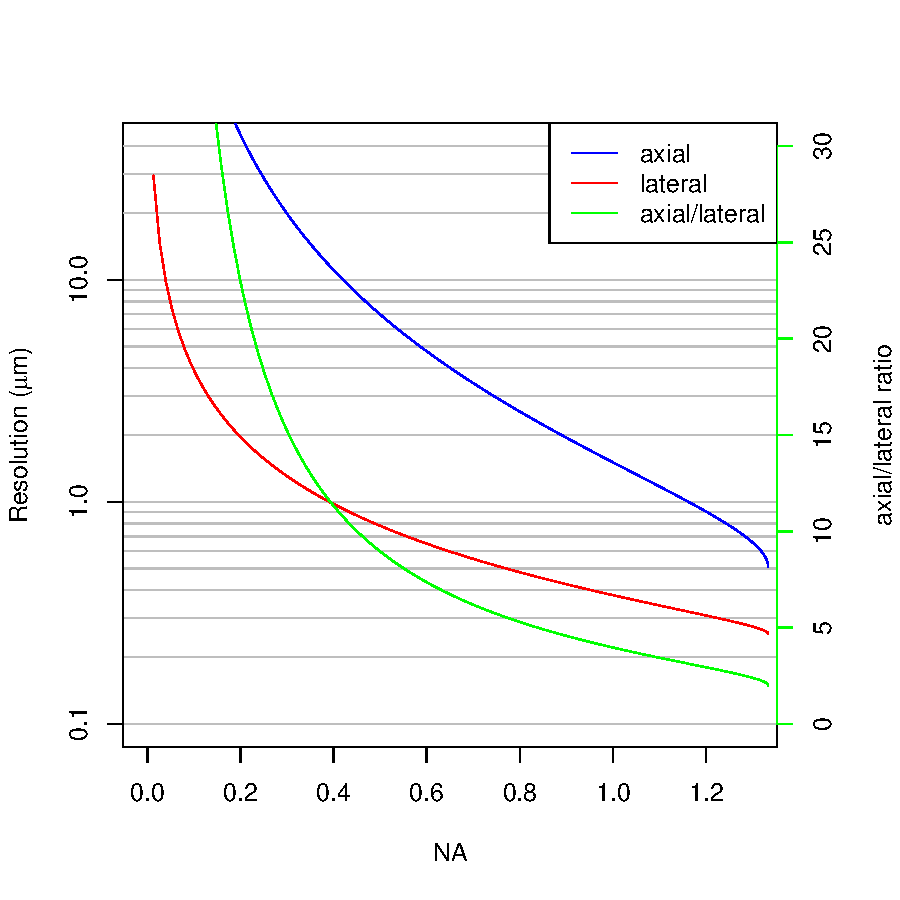
\includegraphics[width=0.6\textwidth]{figures/1_spim/resolution}
    \caption{\textbf{Resolution of a wide-field microscope.} Axial (blue) and lateral (red) resolutions of a wide-field microscope are shown with respect to the numerical aperture (NA). Resolutions are calculated with $\lambda =510nm$, the emission maximum of GFP and $n=1.333$, the refractive index of water, for water dipping objectives.}
    \label{fig:resolution}
\end{figure}

\subsection{Confocal microscopy}

Laser scanning confocal microscopy \cite{davidovits_photomicrography_1973} addresses the problem of noise originating from the out of focus planes. The principle for illumination and detection optics is very similar to a wide-filed microscope, but for illumination a focused laser light is used.

The biggest change is in the detection method: the confocal microscope uses a pinhole, to exclude light coming from out of focus planes. Since only those rays are taking part in the imaging that originate from the focus, the image quality is highly improved. This microscopy technique is also capable of 3D imaging, with an axial resolution corresponding to a wide-filed microscope.

However, the image can not be registered as simply as with the wide-filed detection, since at any given time, only a very small portion of the sample will be used in the imaging. Because of this, a more sensitive detection is required, which generally means the use of a photomultiplier. To get the whole image, the focus is scanned through the whole sample (or rather, the sample is scanned through the focus), recording an intensity value for each position. The image is then generated using a computer based on the recorded position and intensity values.


Although this microscopy technique already has 3D capabilities, it's axial resolution is still limited by the SGH theory, since it uses only one objective. Imaging live specimens for an extended period of time with confocal microscopy although possible \cite{aldaz_live_2010}, is not ideal. Since for each voxel imaged, almost the entire specimen has to be illuminated, which results in a very high dose of radiation of the samples. This can be as much as 30--100 times bigger, than the dose used for the actual imaging \cite{reynaud_light_2008}. High power of laser for an extended time frame can result in bleaching the fluorophores, thus resulting in a lower signal at later times, but the more significant issue is phototoxicity, that is when the cells themselves are damaged by the laser light.

\begin{figure}
\begin{subfigure}[t]{0.49\textwidth}
    \centering
    \includegraphics[page=3,width=\textwidth]{figures/1_spim/spim_cyl}
    \caption{\textbf{Confocal microscope}}
    \label{fig:confocal}
\end{subfigure}
\begin{subfigure}[t]{0.49\textwidth}
    \centering
    \includegraphics[page=5,width=\textwidth]{figures/1_spim/spim_cyl}
    \caption{\textbf{Confocal-theta microscope}}
    \label{fig:conf-theta}
\end{subfigure}
\caption{\textbf{Basic optical components of a laser scanning confocal and confocal-theta microscope.} Both type of microscopes use confocal images detection, which means that a pinhole is used to exclude light coming from out of focus points. Light intensity is measured by a photomultiplier for every voxel in the region of interest. The final image is generated on a computer using the positions and recorded intensity values. A regular confocal microscope (\ref{fig:confocal}) uses the same objective for illumination and detection, while a confocal-theta microscope (\ref{fig:conf-theta}) uses a second objective that is rotated by $\vartheta$ around the focus. In this case, $\vartheta = 90^\circ$.}
\label{fig:confocals}
\end{figure}

\subsection{Confocal-theta microscopy}

Although confocal microscopy already provides a better resolution in all dimensions, the ratio of the axial and lateral resolution is still very high, due to the single objective illumination and detection. This seriously limits the microscope's 3D imaging capabilities, since in the $z$ direction (i.e. along the imaging axis) the resolution would be significantly worse than in the other directions.

Confocal-theta microscopy \cite{stelzer_fundamental_1994} introduces a second objective to a regular confocal microscope, that is used to illuminate the sample (Figure \ref{fig:conf-theta}). Since this decouples the illumination and detection, using a filter cube is no longer necessary. The second objective is rotated by $\vartheta$ around the focus, this is the where the name of this setup originates.

Resolution is also improved compared to the regular confocal microscope, because the lateral resolution of the imaging objective now corresponds to the axial resolution of the detection objective. The combined resolution of the two-objective system can be calculated in the following manner \cite{krzic_multiple-view_2009}:
\begin{equation}
\frac{1}{\sigma _{sys}^2} = \frac{1}{\sigma _{ill}^2} + \frac{1}{\sigma _{det}^2}
\end{equation}
where $\sigma_{ill} = \sigma_{xy}$ and $\sigma_{det} = \sigma_z$ for the axial resolution of the system, and reversed for the lateral resolution of the system. This means, that the axial and lateral resolution would be the same (if the same objectives are used), and the resulting point spread function is almost isotropic.

Although this is a big improvement to confocal microscopy, the issue of photobleaching and phototoxicity is still not solved with a confocal theta microscope, which means that longer developmental processes are near impossible to follow with this type of microscopy.




\section{Light-sheet microscopy}
\label{sec:light-sheet}
One main drawback of the point scanning methods introduced in the previous section is the inefficiency of the illumination scheme. Although almost the whole sample is illuminated, information is only collected from the focal volume. This results in two main limiting factors: acquisition speed depends on the point scanning speed, which in turn is inversely proportional to the signal to noise ratio. Furthermore, because of the inefficiency of the illumination scheme, photobleaching and phototoxic effects further reduce the usability of these techniques for live imaging, especially for long term experiments \cite{}.



The main principle behind single plane illumination microscopy, that is illuminating the sample from the side by a very thin light-sheet, dates back to the early 20\textsuperscript{th} century, when Siedentopf and Zsigmondy first described the ultramicroscope \cite{siedentopf_uber_1902}. This microscope used sunlight as an illumination source, that was guided through a precision slit to generate a thin light-sheet. This allowed Zsigmondy to visualize gold nanoparticles floating in and out of the light-sheet. Since these particles are much smaller than the wavelength of the light, the device was called an ultramicroscope. His studies with colloids together with the development of the ultramicroscope led Zsigmondy to win the Nobel Prize in 1925.

previous to SPIM:
Voie et al. fixed guinea pig cochlea, rotating and reconstruction in 3D \cite{voie_orthogonal-plane_1993}, called Orthogonal-plane Fluorescent Optical Sectioning. Lateral resolution around \SI{10}{\micro m} and axial resolution of \SI{26}{\micro m}, with very large, \SI{1.5}{mm} field of view. Since the specimens they imaged contained calcium rich bone tissue, optical imaging was only possible by using an optical clearing method. In this work, they used EDTA (ethylenediaminetetraacetic acid) dehydrated in ethyl alcohol, then it was cleared, finally immersed in a fluorescent dye bath. TO acquire 3D images, the specimen was rotated, and translated to compensate for the off-axis rotation.

follow-up to Voie and Spelman: \cite{voie_three-dimensional_1995} 3D reconstruction of the cochlea for the images

Similar to SPIM but not fluorescent: light scanning photomicrography \cite{huber_3d_2001}

Then, in 2002, Fuchs et al. introduces Thin  Light-Sheet Microscopy \cite{fuchs_thin_2002} who use this technique to investigate the microbial life in seawater samples without disturbing their natural environment (by e.g. placing them on a coverslip). Using TSLM allowed the to image the bacteria directly in the staining solution containing SYBR Green I without having to deal with background illumination from the dye, which would have been an issue with confocal microscopy for example. Their light-sheet was similar to the one utilized in OPFOS, being \SI{23}{\micro m} thin, and providing a \SI{1}{mm} \ \SI{1}{mm} field of view.

The real breakthrough happened when light-sheet microscopy was combined with 
endogenous fluorescent labels: fluorescent proteins
live imaging for long time
and light-sheet
these techniques were all combined in the 2004 Science paper from Huisken et al. that marks a landmark in light-sheet microscopy, and since then a widespread adoption started  in biological research, with multiple groups implementing their own setups.

Since then however, light-sheet microscopy was seldom used, but in the last decade it was reinvented and combined with fluorescent microscopy. The first notable light-sheet fluorescent microscope (LSFM) was developed at EMBL in 2004 \cite{huisken_optical_2004}, that demonstrated the benefits of using a light-sheet in imaging developmental processes in three dimension.

Since then, light-sheet based imaging has gained more and more popularity, as it can be adapted and applied to a wide variety of problems. It was numerously proven to be a better choice than confocal microscopy \cite{reynaud_light_2008,huisken_selective_2009} especially in developmental biological applications \cite{weber_light_2011}. It can also be used with a wide variety of specimens of different sizes, such as zebrafish embryo \cite{keller_reconstruction_2008}, mouse brain \cite{dodt_ultramicroscopy:_2007} or drosophila embryo \cite{krzic_multiview_2012}. It is also possible to use light-sheet microscopy in super-resolution, allowing for individual molecule localization \cite{cella_zanacchi_live-cell_2011}.

%\begin{itemize}	
%	\item mSPIM, pivoting light-sheet \cite{huisken_even_2007}
%	\item omnidirectional microscopy (review) \cite{weber_omnidirectional_2012}
%	\item SiMView \cite{tomer_quantitative_2012}
%\end{itemize}

\section{Optics of light-sheet microscopy}

A selective-plane illumination microscope (SPIM) uses a light-sheet to illuminate only a thin section of the sample (Figure~\ref{fig:light-sheet}). This illumination plane is perpendicular to the imaging axis of the detection objective and coincides with the focal plane. This way the image is taken of only that specific plane that is illuminated, thus providing much better signal to noise ratio. In case of conventional wide-field fluorescent microscopy, where the whole specimen is illuminated, light scattering from different regions contribute to a significant background noise. With selective-plane illumination, this problem is intrinsically solved, and it also provides a true sectioning capability. This makes SPIM especially suitable for 3D imaging.



\begin{figure}[htpb]
    \centering
    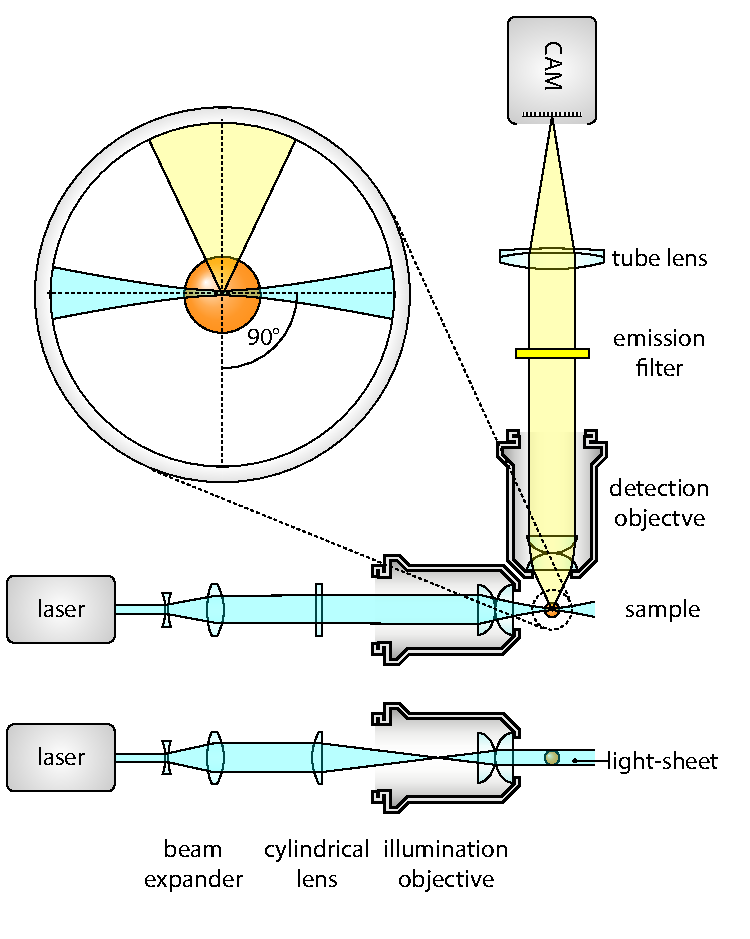
\includegraphics[page=1,width=0.8\textwidth]{figures/1_spim/spim_cyl}
    \caption{\textbf{Basic optical components of a SPIM.} A selective plane illumination microscope uses two objectives orthogonally aligned. One objective is used to generate a thin light-sheet that illuminates the sample from the side, while the other is used for detection. To generate an image of the specimen, a suitable tube lens is used to focus the light on the sensor of a detection unit (e.g. sCMOS camera). The light-sheet is generated by the illumination objective, using a beam that is previously shaped by a cylindrical lens.}
    \label{fig:light-sheet}
\end{figure}


\subsection{Detection}
The detection unit of a SPIM is basically equivalent to a detection unit of a wide-field microscope, without a dichroic mirror (Figure \ref{fig:light-sheet}). Most important components are the objective together with the tube lens, filter wheel, and a sensor, typically a CCD or sCMOS camera.

One of the most important aspects that determine the resolution of the microscope is the detection objective. Since in developmental biology specimens require a water-based solution, these objectives are usually water dipping objectives directly submerged in the medium. Since the refraction index of water ($n=1.333$) is greater than the refraction index of air, these objectives tend to have a higher $NA$, which results in higher resolution. This, however, also depends on the sensor used, mainly on the pixel size ($d_{sensor}$).

The magnification is typically $10\times$, $20\times$, $40\times$ or $100\times$ but these values are sound only when the objective is used together with the prescribed tube lens. These lenses are specially made to be used with the specific objectives, and are corrected for any aberrations. They typically have a focal length of 160--200mm.

\subsection{Illumination}

\subsubsection{Using cylindrical lens}
The light-sheet can be generated using a cylindrical lens, which focuses the laser beam in only one direction, and creating a thin sheet in the proximity of the focal point. However, to achieve light-sheets that are thin enough, one would need to use cylindrical lens with low focal lengths, but these are hardly accessible in well corrected formats. For this reason, its more common to use a longer focal length cylindrical lens in conjunction with a microscope objective, which is well corrected for chromatic and spherical aberrations \cite{greger_basic_2007}. This way, the light-sheet length, thickness and width can be adjusted for the specific imaging tasks.

For paraxial waves, i.e. waves with nearly parallel wave front normals, a general wave equation can be approximated with the paraxial Helmholz equation \cite{krzic_multiple-view_2009, saleh_fundamentals_2007}
\begin{equation}
    \nabla_T^2 + i 2k \frac{\partial U}{\partial z} = 0
    \label{eq:helmholtz}
\end{equation}
where $\nabla_T^2 = \frac{\partial^2}{\partial x^2} + \frac{\partial^2}{\partial y^2}$, $U(\vec{r})$ is the wave-function, $k=\frac{2\pi}{\lambda}$ is the wavenumber and we assume, that the light spreads in $z$ direction.
 
A simple solution to this differential equation is the Gaussian beam:
\begin{equation}
    U(r,z) = A_0 \cdot \frac{W_0}{W(z)} \cdot e^{-\frac{r^2}{W^2(z)}}\cdot e^{-i\cdot \phi(r,z)}
\label{eq:gaussian}
\end{equation}
where $A_0$ is the amplitude of the wave, $W_0$ is the radius of the beam waist (the thinnest location on the beam), $r=\sqrt{x^2+y^2}$ is the distance from the center of the beam, $W(z)$ is the radius of the beam $z$ distance from the waist, and $\phi(r,z)$ is the combined phase part of the wave-function. Furthermore:

\begin{equation}
    W(z) = W_0\sqrt{1+\left( \frac{z}{z_0} \right)^2}
\end{equation}
where the parameter $z_0$ is called the Rayleigh-range. This has the following connection with the beam waist:

\begin{equation}
    z_0 = \frac{\pi W_0}{\lambda}
\end{equation}
Which means, the thinner the beam waist, the shorter the Rayleigh-range, that is the beam divergence is faster for more focused beams.

Intensity of the emitted fluorescence is based on the intensity of the excitation light. In case of a Gaussian beam:
\begin{equation}
    I(r,z) = U(r,z)\cdot U^*(r,z) = |A_0|^2 \cdot \left( \frac{W_0}{W(z)}\right)^2 \cdot e^{-\frac{2r^2}{W^2(z)}}
\end{equation}

Apart from the circular Gaussian beam, the elliptical Gaussian beam is also an eigenfunction of Helmholtz equation (\ref{eq:helmholtz}):
\begin{equation}
    U(x,y,z) = A_0 \cdot \sqrt{\frac{W_{x,0}}{W_x(z)}} \sqrt{\frac{W_{y,0}}{W_y(z)}} \cdot e^{-\frac{x^2}{W_x^2(z)}} \cdot e^{-\frac{y^2}{W_y^2(z)}} \cdot e^{-i\cdot \phi(x,y,z)}
\end{equation}

This beam still has a Gaussian profile along the $x$ and $y$ axes, but the radii are uncoupled, which results in an elliptical beam. Since the beam waist is different along the two axes, the Rayleigh range is also different:
\begin{align}
    z_{x,0} = \frac{\pi W_{x,0}^2}{\lambda} \\
    z_{y,0} = \frac{\pi W_{y,0}^2}{\lambda}
\end{align}
Intensity of the beam is the following:
\begin{equation}
    I(x,y,z) = U(x,y,z)\cdot U^*(x,y,z) = |A_0|^2 \cdot \frac{W_{x,0}}{W_x(z)} \cdot \frac{W_{y,0}}{W_y(z)} \cdot e^{-\frac{2x^2}{W_x^2(z)}} \cdot e^{-\frac{2y^2}{W_y^2(z)}}
\end{equation}
where
\begin{align}
W_x(z) = W_{x,0}\sqrt{1+\left( \frac{z}{z_{x,0}} \right)^2}\mathrm{\quad and \quad } W_y(z) = W_{y,0}\sqrt{1+\left( \frac{z}{z_{y,0}} \right)^2}
\end{align}

Since the illumination is uneven, the usable field of view is smaller than the actual illuminated region (Figure \ref{fig:fov}). The width of the field of view $w_{fov}$ is determined by the Rayleigh length, since this is in a direct relation with the beam divergence. To stay in the optimal region, the light-sheet should only be used in the range of 1 Rayleigh length on both sides of the beam waist (Figure \ref{fig:width}). In this range, the ratio between the thickest (at $z=z_0$) and the thinnest (at $z=0$) part of the beam $W(z)$ will be $\sqrt{2}\approx 1.4142$ which is still acceptable.

Light-sheet height is determined by the profile of the beam along the vertical axis (Figure \ref{fig:height}). Since this is a Gaussian function (see Equation \ref{eq:gaussian}), only a small part in the middle can be used for imaging, because towards the sides the intensity dramatically drops. To allow a maximum 80\% drop of intensity at the edges, the light-sheet height is $h_{fov}=2\cdot 0.472\cdot W_{x,0}$
\begin{figure}[b!]
    \centering
    \begin{subfigure}[b]{0.7\textwidth}
        \centering
        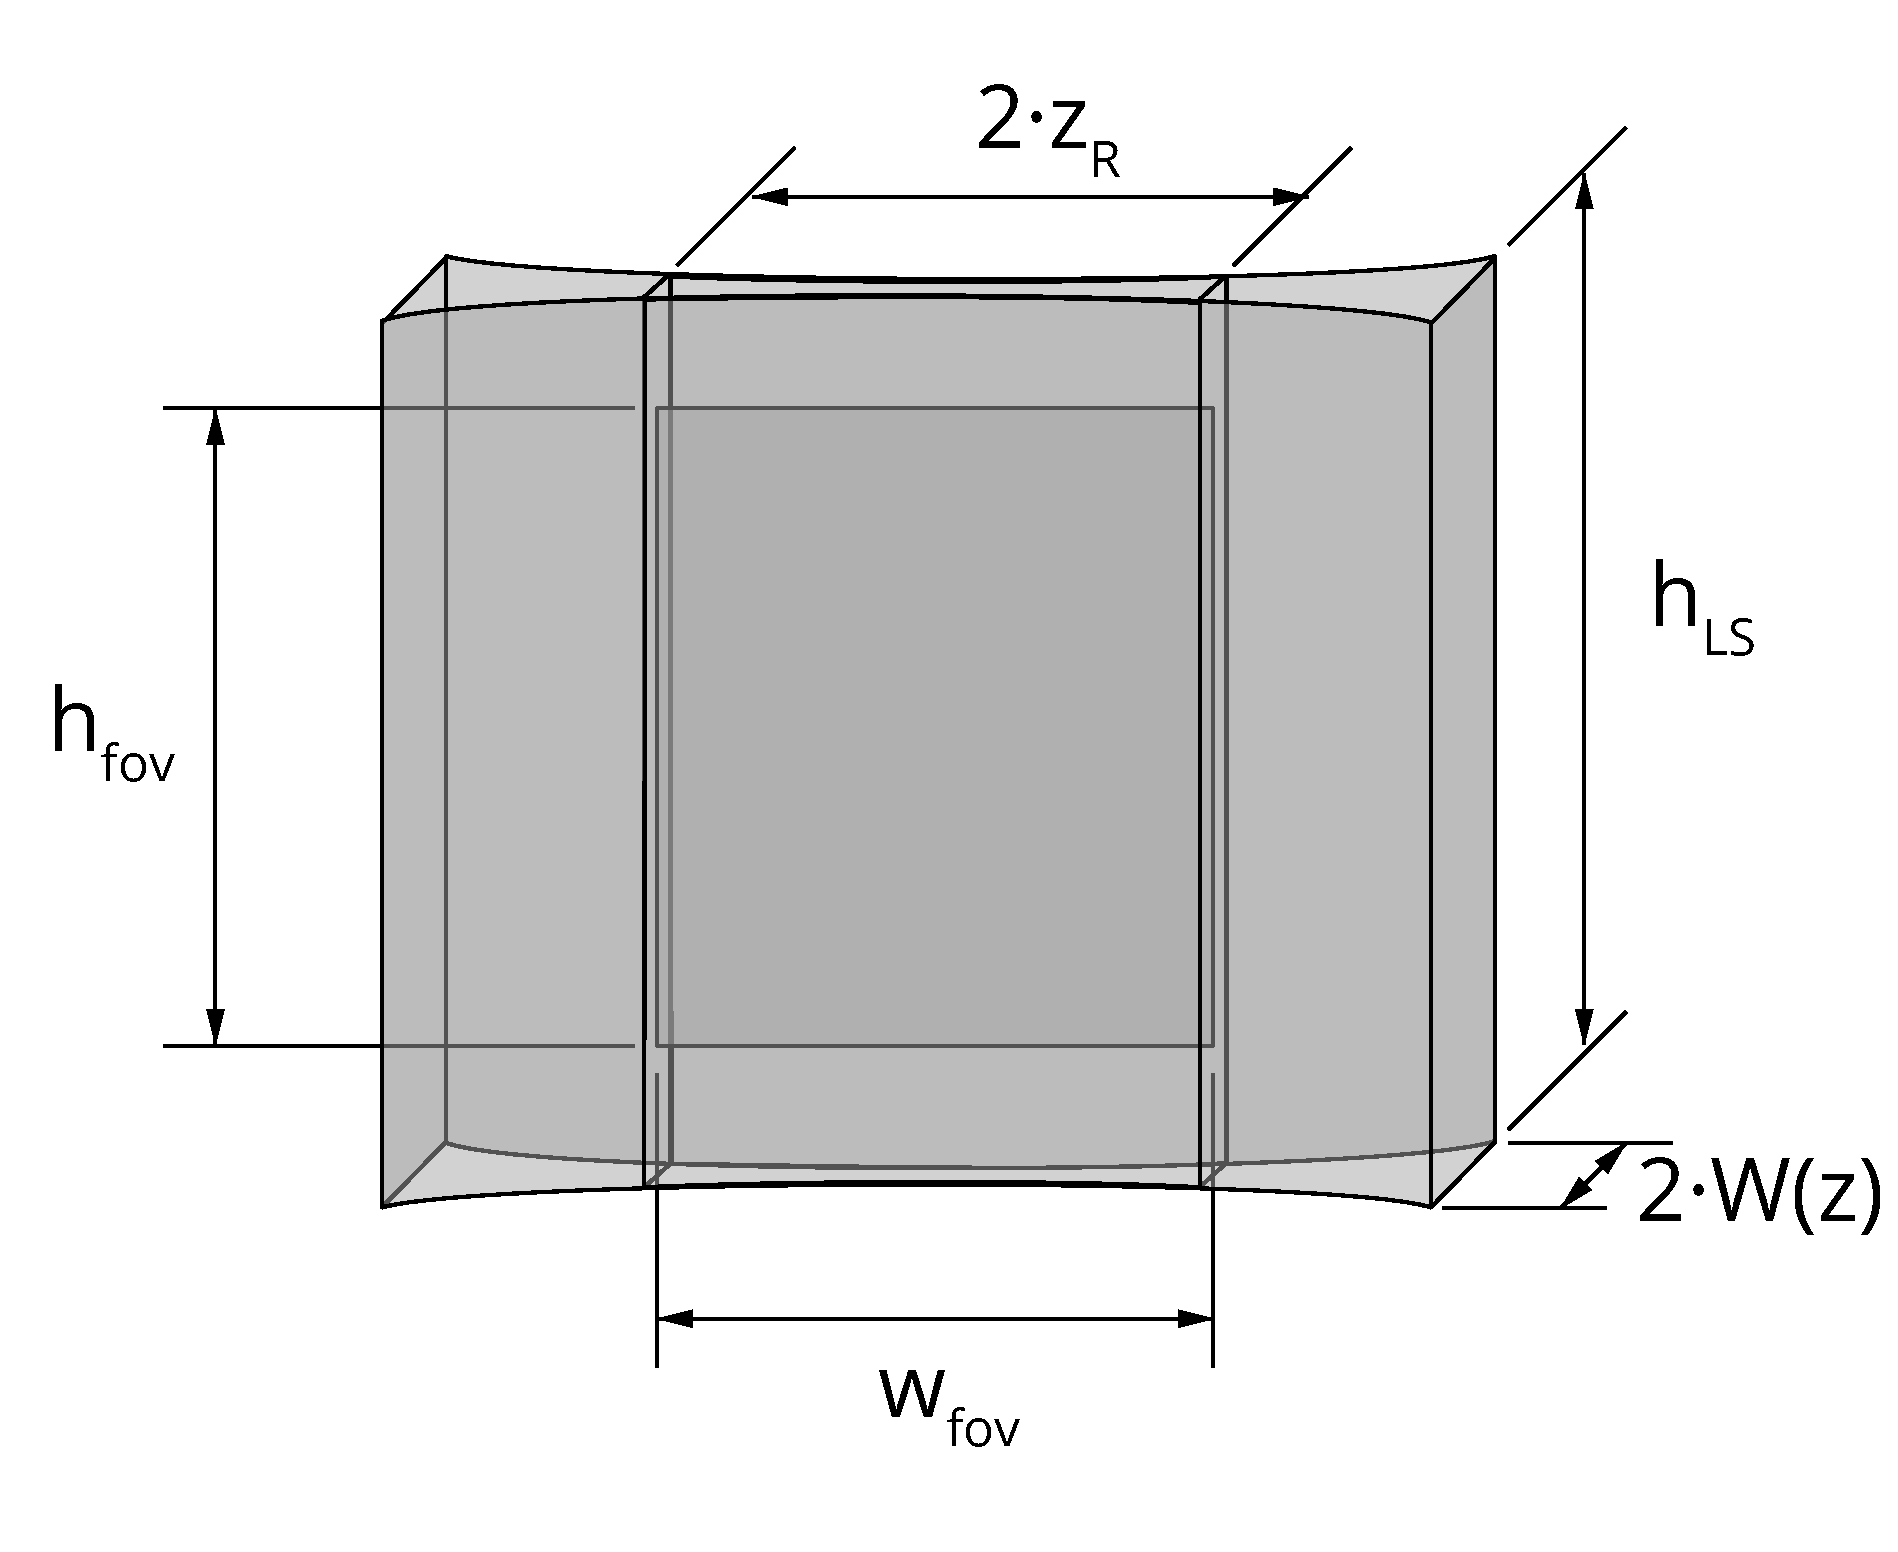
\includegraphics[width=\textwidth]{figures/1_spim/FOV}
        \caption{}
        \label{fig:fov}
    \end{subfigure}
    \begin{subfigure}[b]{0.49\textwidth}
        \centering
        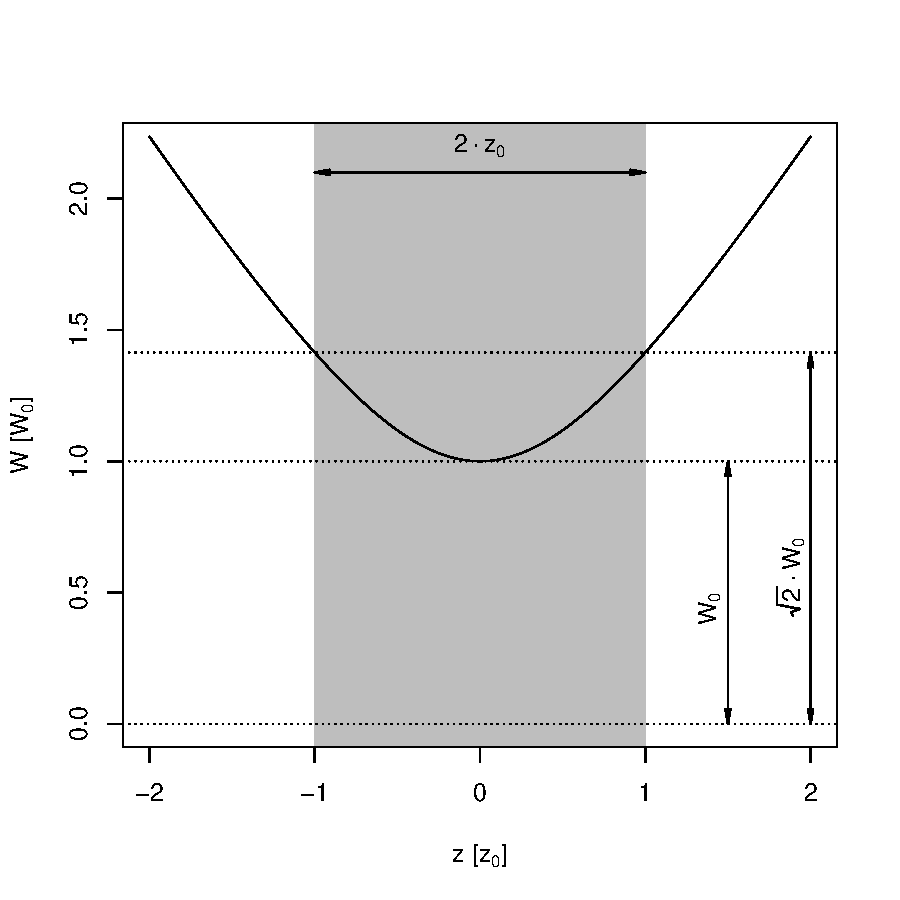
\includegraphics[width=\textwidth]{figures/1_spim/width}
        \caption{}
        \label{fig:width}
    \end{subfigure}
    \begin{subfigure}[b]{0.49\textwidth}
        \centering
        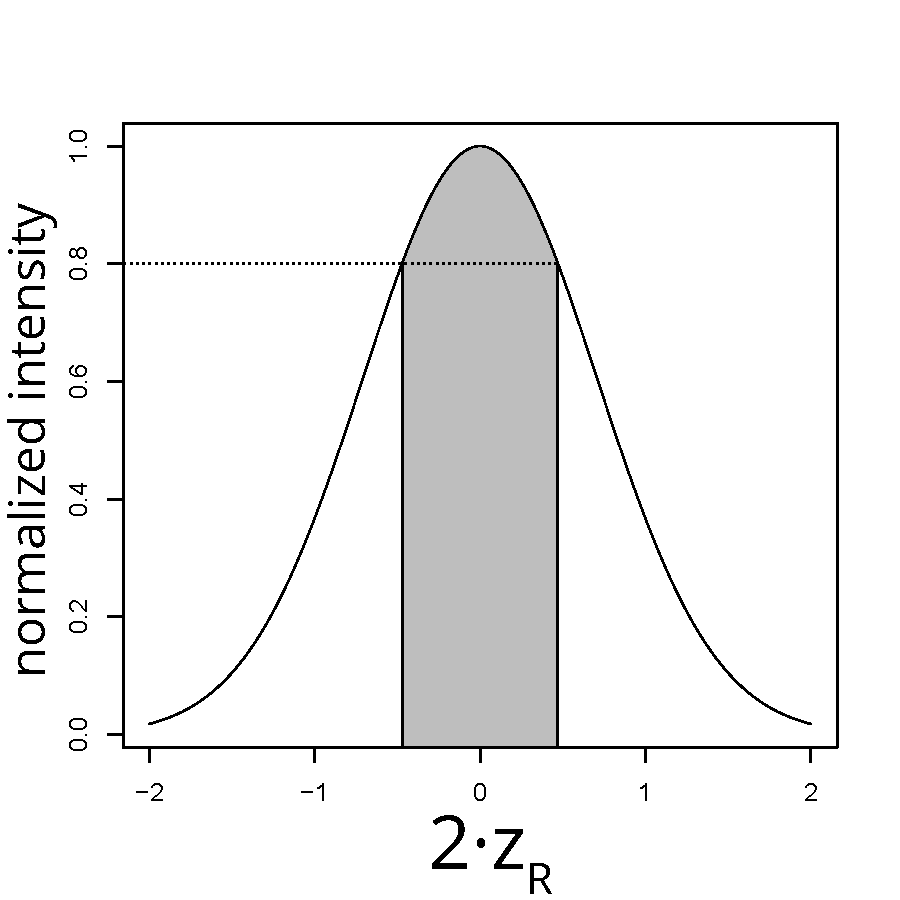
\includegraphics[width=\textwidth]{figures/1_spim/height}
        \caption{}
        \label{fig:height}
    \end{subfigure}
    \caption{\textbf{Light-sheet dimensions.} \ref{fig:fov} shows a light sheet, with the field of view indicated. Since the light-sheet intensity is uneven, the field of view has to be confined to a smaller region. \ref{fig:width} The width and thickness of the field of view depends on the Rayleigh length of the beam ($z_{y,0}$). \ref{fig:height} Height of the field of view is determined by the Gaussian profile of the elliptical beam.}
    \label{fig:ls_dim}
\end{figure}

\subsubsection{Using focused beam scanning}
\begin{figure}[hbt]
    \centering
    \includegraphics[page=2,width=0.8\textwidth]{figures/1_spim/spim_cyl}
    \caption{\textbf{DSLM illumination.} DSLM illuminates a specimen by a circularly-symmetric beam that is scanned over the field of view. This creates a virtual light-sheet, which illuminates a section of a specimen just like the SPIM. Light-sheet in DSLM is uniform over the whole field of view and its height can be dynamically altered by changing the beam scan range.
}
    \label{fig:dslm}
\end{figure}

Since using cylindrical lenses it's not possible to generate a homogeneous light-sheet, moreover at higher magnification the Rayleigh range would be too small, we also consider using focused beam scanning to generate the light-sheet (digital scanned light-sheet microscopy, DSLM). To generate a scanning beam, a galvanometer controlled mirror is used to alter the beam path. This can quickly turn around its axis which will result in an angular sweep with the laser beam. To change the angular movement to translation, a scan lens is used to generate an intermediate scanning plane. This plane is then imaged to the specimen by the tube lens and the illumination objective, resulting in a scanned focused beam.

This method to generate the light-sheet has several advantages compared to a static light-sheet. The height of this sheet is not determined by the cylindrical lens, but it can be dynamically modified. Also, the intensity is uniform through the whole height of the light-sheet.

\section{Multi-view light-sheet microscopy}
already in 1989 multi-view to increase axial resolution in conventional optical microscope. They imaged \textit{Drosohpila} metaphase plate in Zeiss Axiomat microscope using a 63x 1.2 NA water immersion objective lens. To increase the axial resolution, a special rotation stage was constructed, that allowed rotation around the object of interest to image it from a 90\si{\degree} tilted view. Using a fusion method in the Fourier space, the resolution increased to \SI{0.25}{\micro\meter} in lateral and \SI{0.4}{\micro\meter} in the axial direction for real samples.

Multiple imaging axis microscopy (MIAM) \cite{swoger_multiple_2003}
to image specimens from 4 directions in a tetrahedral objective configuration, could reach a 5.8 fold increase in axial resolution by combining the four views as a weighted average.
Follow up for this: sample manipulation with optical tweezers / optical levitation in 3D \cite{huisken_three-dimensional_2007}(because of the lack of space for mechanical translation stage)
positioning of a \SI{20}{\micro m} latex bead in a \SI{100}{\micro m} diameter volume by changing the intensity of 4 laser beams. 

\section{SPIM improvements}
things to improve: resolution
axial resolution relative to lateral
complete view
reduce scattering

\chapter{Dual Mouse-SPIM}
    \section{Previous Mouse-SPIM}
    \section{Light collection efficiency of an objective}
    Resolution is not the only parameter of concern when designing a new microscope setup. We also have to consider light collection efficiency, since many application, especially live imaging applications require a tight photon budget. This means a single fluorophore can only emit so many times before it undergoes an irreversible chemical reaction, i.e. it bleaches. The more we can collect of these photons, the more information we gain, and altogether the efficiency is higher.
    
    Photon collection efficiency also defines single molecule localization accuracy, since the signal to noise ratio will depend on the square of the number of collected photons. This is why it's important to also maximize light collection efficiency.
    
    Let's define light collection efficiency $\eta$ as the ratio of collected photons and all emitted photons:
    \[
    \eta = \frac{N_{collected}}{N_{emitted}}
    \]
    Since we can assume that the direction of photons emitted from a fluorescent molecule are random, the light collection efficiency will correspond to the solid angle subtended by the objective front lens at the focal point. To calculate this, let's consider the unit sphere centered at the focal point, and calculate the surface area of the spherical cap corresponding to the objective acceptance angle $\alpha$ (Fig. \ref{fig:light_effa}). The area of the cap can be expressed as a function of the angle:
    \[
    A_{cap} = 2\pi r^2 (1-\cos \alpha)
    \]
    The surface area of the full sphere is calculated as:
    \[
    A_{sph} = 4 \pi r^2
    \]
    For both equations $r$ is the radius of the sphere. From here, the light collection efficiency can be calculated as:
    \[
    \eta = \frac{N_{collected}}{N_{emitted}} = \frac{A_{cap}}{A_{sph}} = \frac{1-\cos \alpha}{2}
    \]

Some more calculations: (Fig. \ref{fig:light_effb}).

\begin{figure}[tpb]
\begin{subfigure}[t]{0.49\textwidth}
    \centering
    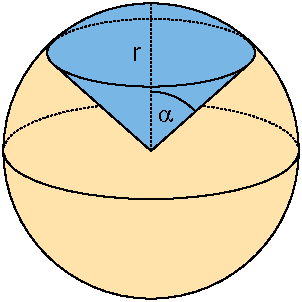
\includegraphics[page=1,width=0.8\textwidth]{figures/2_DualMouse/efficiency/sphere}
    \caption{\textbf{}}
    \label{fig:light_effa}2
\end{subfigure}
\begin{subfigure}[t]{0.49\textwidth}
    \centering
    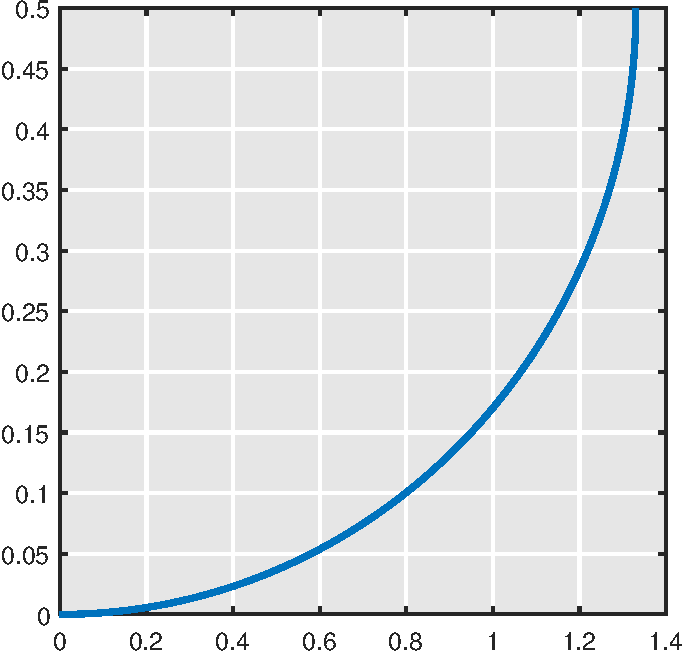
\includegraphics[page=1,width=1\textwidth]{figures/2_DualMouse/efficiency/light_eff}
    \caption{\textbf{}}
    \label{fig:light_effb}
\end{subfigure} 
 \caption{\textbf{Light collection efficiency of an objective.} \textbf{(a)} Light collection efficiency is the ratio of photons collected by the objective and all emitted photons. If the fluorophores are emitted randomly in all directions, it will be the surface ratio of the conical section (blue) to the whole sphere. \textbf{(b)} Light collection efficiency ($\eta$) as a function of the numerical aperture (NA)}
 \label{fig:light_eff}
\end{figure}


    
    
    
    \section{3D figure test}
    
\begin{figure}[htb]
\centering
    \includemedia[
    width=0.8\linewidth,height=0.6\linewidth,
    %add3Djscript=asylabels.js, %upright text labels
    %add3Djscript=3Dspintool.js, %let scene rotate about z-axis
    % 3Dcoo, 3Droo values found with `Generate Default View' from
    % context menu
    3Dmenu,
    playbutton=plain,
    3Droll=124.45821807473328,
    3Dc2c=0.5729350447654724 0.4988637864589691 0.6502924561500549,
    3Dcoo=6.723448276519775 -30.282148361206055 -11.914359092712402,
    3Droo=162.71372963736036,
    3Dlights=Headlamp,
    3Drender=ShadedIllustration,
    ]{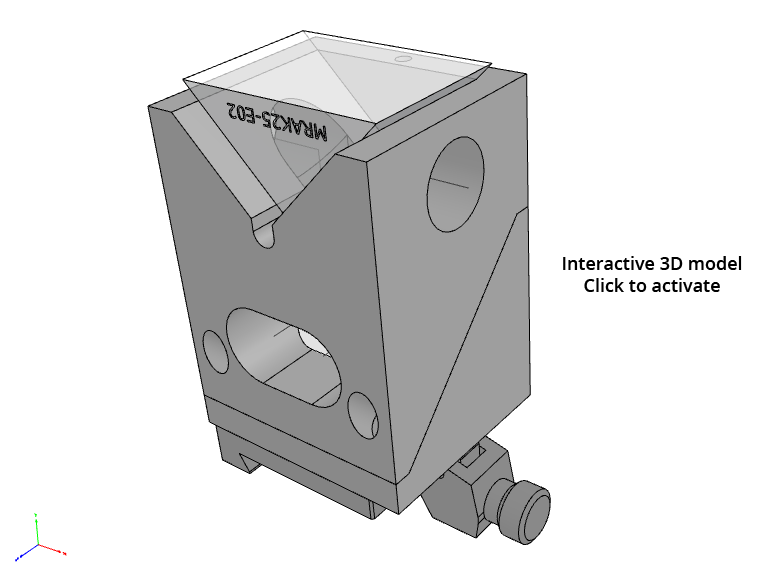
\includegraphics{figures/2_DualMouse/Splitter.png}}{figures/2_DualMouse/Splitter.prc}
\caption{\textbf{Illumination branch splitting block.} 3D model of the custom designed splitter block used in the illumination branch. Depending on the horizontal beam position at the lower port, the beam will be reflected either to the right or to the left. Because of the mirror alignment, the beam is rotated 90 degrees.}
\label{fig:splitter}
\end{figure}


\begin{figure}[htb]
\centering
    \includemedia[
width=1.0\linewidth,height=0.6\linewidth,
%add3Djscript=asylabels.js, %upright text labels
%add3Djscript=3Dspintool.js, %let scene rotate about z-axis
% 3Dcoo, 3Droo values found with `Generate Default View' from
% context menu
3Dmenu,
playbutton=plain,
% default view start
3Droll=104,
3Dc2c=0.7466059923171997 0.4799830913543701 0.4606471359729767,
3Dcoo=-5.2039947509765625 -5.257904529571533 23.018417358398438,
3Droo=353,
3Dlights=Headlamp,
3Drender=ShadedIllustration,
% default view end
]{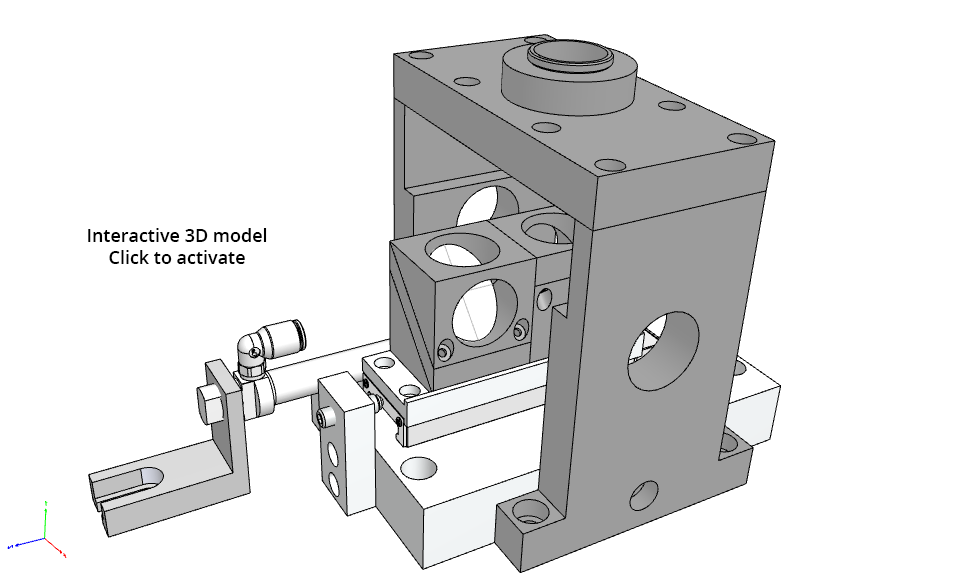
\includegraphics{figures/2_DualMouse/DualMirror.png}}{figures/2_DualMouse/DualMirror.prc}
\caption{\textbf{Detection branch merging unit.} 3D model of the custom designed unit to enable quick switching between the two detection paths. A high precision stainless steel stage holds two mirror blocks facing opposite directions, and bouncing the light upwards, towards the camera. The units are translated by  pneumatic cylinder to ensure high speed an reproducibility.}
\label{fig:DualMirror}
\end{figure}	

\section{Optical layout}

\begin{figure}[hbt]
    \centering
    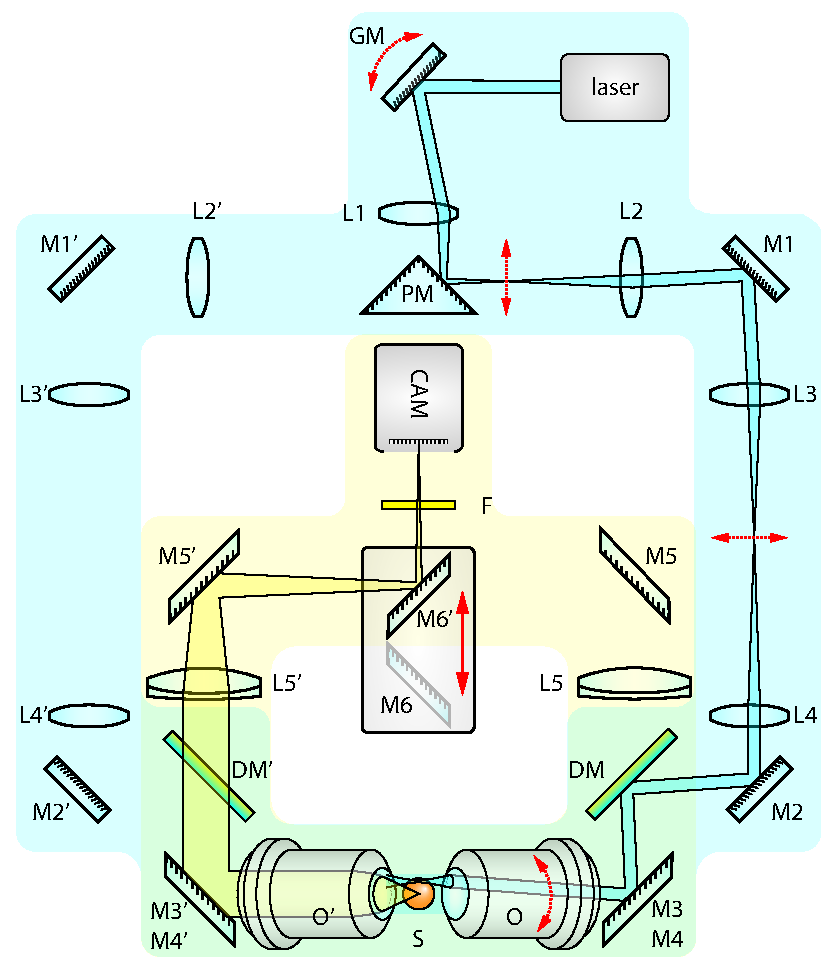
\includegraphics[page=1,width=1\textwidth]{figures/2_DualMouse/fullSchematics}
    \caption{\textbf{Dual Mouse SPIM optical layout.} The microscope consists of two main parts, the illumination branch (blue) and detection branch (yellow). For both illumination and detection there are two identical paths implemented, that can be chose by either the galvanometric mirror (G), or the pneumatic switcher unit (SW). 
}
    \label{fig:fullSchematics}
\end{figure}

    
\chapter{Image processing}

When using any kind of microscopy in research, image processing is a crucial part of the workflow. This is especially true for light-sheet microscopy, since it's capable imaging the same specimen for multiple days, producing immense amounts of data. A single overnight experiment of \textit{Drosophila} development (which is a very typical use-case for light-sheet) can produce multiple terabytes of data. To see the real scales, let's consider the following imaging conditions:
\begin{center}
\begin{tabular}{rl}
    camera & Hamamastu Orca Flash 4 \\
    image size & 8 MB \\
    1 stack = 250 planes & 2 GB \\
    2 views & 4 GB \\
    Time-lapse: 16 h @ 2/min & 7.5 TB \\
    $n$ colors & $n\cdot 7.5$ TB
\end{tabular}
\end{center}

As it is apparent from this table, 


proportional to the symbol frequencies. A string of symbols can be encoded by applyingthis process recursively: The sub-interval from the previous step is subdivided againusing the same proportions. Figure4.2. shows an example of arithmetic coding using

\section{Multi-view fusion techniques}
    \subsection{Why multi view}
    
    \subsection{registration}
        \subsubsection{Image based registration}
        \subsubsection{Bead based registration}
        \subsubsection{Affine transformation}
    \subsection{fusion}
        \subsubsection{Average}
        \subsubsection{Sigmoidal weighted average}
        \subsubsection{Fourier mixing}
        Huisken had something like this
        \subsubsection{Wavelet-based fusion}
        \subsubsection{Multi-view deconvolution}
        
        \cite{krzic_multiple-view_2009} Uros thesis
        \cite{temerinac-ott_multiview_2012}, \cite{temerinac-ott_spatially-variant_2011} Spatially variant deconvolution
        
        
\section{Image compression}
Image compression is an important tool for everyday life, however it's rarely used in the context of scientific imaging because of fear of information loss. This preconception is mainly due to the famous blocking artifacts found in many highly compressed JPEG images, however not all image compression algorithms introduce artifacts, and in fact many lossless algorithms exist that would be suitable for such images. Nowadays, when data production is in an exponential growth compression is again in highlight, without it it would be extremely difficult to maintain many scientific projects that produce images at a high data rate. 

In this paper I will review the basics of image compression based on Sayood's textbook, Introduction to Data Compression \cite{sayood_introduction_2012}. 
I will introduce some basics of information theory and entropy, followed by discussing two widely used entropy coding algorithms, Huffman coding and arithmetic coding. Section 3 will be about transform coding, specifically Discrete Cosine Transform (DCT) and wavelet transform while also touching upon techniques based on differential pulse code modulation. Finally I will show how some of the most widely used image compression standards use these methods to achieve effective image compression.

\section{Entropy coding}
\subsection{Information and Entropy}
For the purpose of data compression it is useful to quantify the amount of \textit{information} contained within a piece of data. The first rigorous definition of information was presented in an extremely influential paper by Shannon, published in two parts in 1948 \cite{shannon_mathematical_1948, shannon_mathematical_1948-1}.

First, let's define the amount of self-information contained in the outcome of a random experiment:
\begin{equation}
I(A) = \log_b \frac{1}{P(A)} = - \log_b P(A)
\end{equation}

2 independent events:
\begin{equation}
P(A,B) = P(A) \cdot P(B)
\end{equation}

self-information is additive:
\begin{align}
I(A,B) &= \log_b \frac{1}{P(A,B)} \\
&= \log_b \frac{1}{P(A) \cdot P(B)} \\
&= \log_b \frac{1}{P(A)} + \log_b \frac{1}{P(B)}
\end{align}

entropy for random variable $X$ ~ average or expected self-information for the random variable
\begin{equation}
H(X) = \sum_i P(A_i)I(A_i) = - \sum_i P(A_i) \log_b P(A_i)
\end{equation}

entropy rate for data source $S$ ~ average information output by the data source

\subsection{Huffman coding}
Huffman coding is a prefix-free, optimal code that is widely used in data compression. It was developed by David A. Huffman as a course assignment on the first ever course on information theory at MIT, and was published shortly afterwards \cite{huffman_method_1952}. It is a variable length binary code which assigns different length codewords to letters of different probabilities. It is able to achieve optimal compression, which means the total length of the coded sequence will be minimal.

Although it produces a variable length code which can introduce some issues with decoding, it is still uniquely decodable. It achieves this property by using prefix-free codewords, meaning that none of the codewords are prefixes of any other codewords. This property can be exploited when decoding the codeword, since during this procedure the number of bits for the next codeword can not be determined in advance. However if no codeword is a prefix of another codeword, by simply reading the successive bits one by one until we reach a valid codeword, it's possible to uniquely decode the message.

Let's take the example in Table \ref{tab:huffman1}. Five letters are coded in binary code by Code \#1 and by Code \#2. Code 1 is not a prefix code, and because of this when reading the encoded sequence we can not be sure when we reach the end of a codeword. Decoding the sequence 0000 for example could be interpreted as 4 letters of $a_1$ or 2 letters of $a_3$.

\begin{table}
\caption{Examples of a random binary code (\#1) and a prefix-free binary code (\#2). Code \#2 is uniquely decodable, while for code \#1 it's necessary to introduce boundaries between codewords to be able to distinguish them.}
\centering
\begin{tabular}{crr}
\toprule
Letter & Code \#1 & Code \#2 \\
\midrule
$a_1$ & 0	& 10 \\
$a_2$ & 11	& 11 \\
$a_3$ & 00	& 00 \\
$a_4$ & 10 	& 010 \\
$a_5$ & 111	& 011 \\
\bottomrule
\end{tabular}
\label{tab:prefix}
\end{table}

The Huffman coding procedure is based on two observations regarding optimal and prefix-free codes:
\begin{enumerate}
\item For a letter with higher frequency the code should produce shorter codewords, and for letters with lower frequency it should produce longer codewords.
\item In an optimum code, the two least frequent codewords should have the same lengths.
\end{enumerate}

From these statements the first is trivial to see that is correct. If the more frequent letters would have longer codewords then the less frequent letters, the average codeword length (weighted by the probabilities) would be larger than in the opposite case. Thus, more frequent letters must not have longer codewords than less frequent letter.

The second statement at first glance might be so intuitive, so let's consider the following situation. The two least frequent codewords do not have the same lengths, that is the least frequent is longer. However, because this is a prefix code, the second longest codeword is not a prefix of the longest codeword. This means, if we truncate the longest codeword to the same length as the second longest, they will still be distinct codes and uniquely decodable. This way we have a new coding scheme which requires less space on average to code the same sequence as the original code, from which we can conclude the original code was not optimal. Therefore, for an optimal code, statement 2 must be true.

\begin{table}
\caption{Huffman code table}
\centering
\begin{tabular}{ccr}
\toprule
Letter & Probability & Codeword \\
\midrule
$a_2$ & 0.4 & $c(a_2)$ \\
$a_1$ & 0.2 & $c(a_2)$ \\
$a_3$ & 0.2 & $c(a_2)$ \\
$a_4$ & 0.1 & $c(a_2)$ \\
$a_5$ & 0.1 & $c(a_2)$ \\
\bottomrule
\end{tabular}
\label{tab:huffman1}
\end{table}

\begin{figure}
\centering
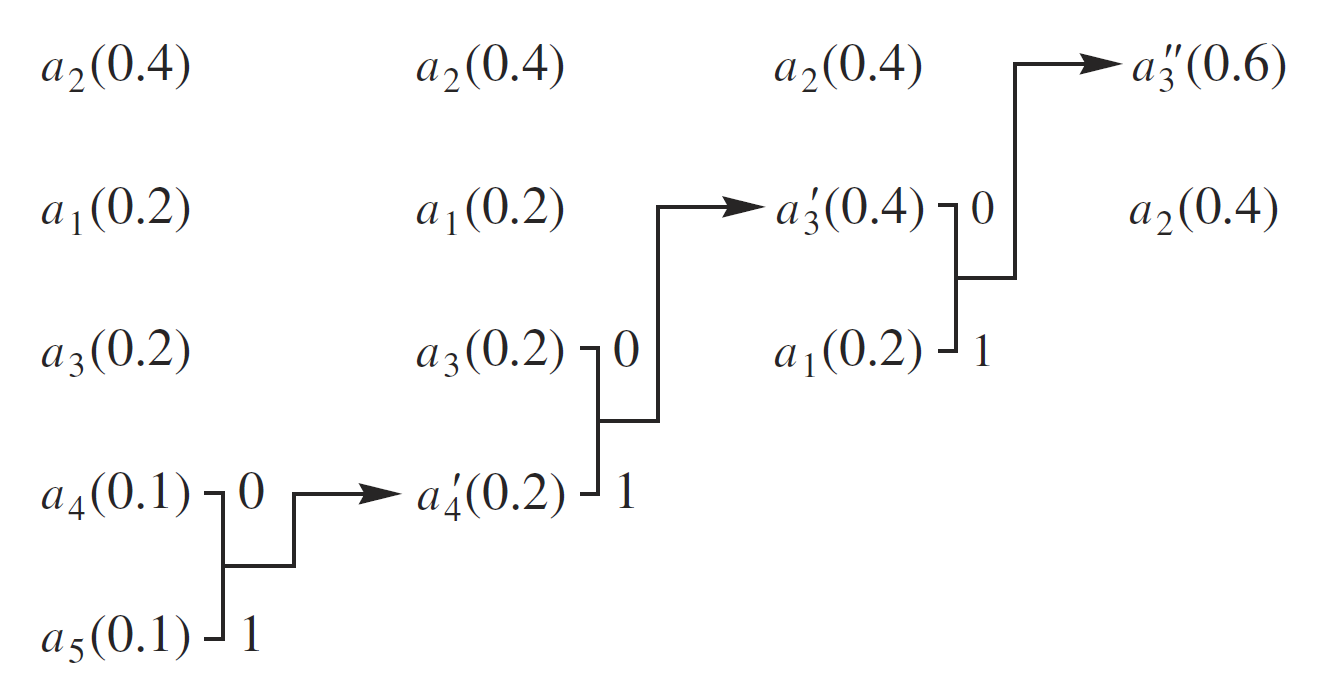
\includegraphics[width=0.6\textwidth]{figures/3_compression/huffman}
\caption{Building the binary Huffman tree. The letters are ordered by probability, these will be the final leave of the tree. To join the to branches at every iteration we join the to nodes with the smallest probability, and create a new common node with the sum of the probabilities. This process is continued until all nodes are joined in a root node with probability of 1. Now, if we traverse down the tree to each leaf, the codeword will be defined by their position. }
\label{fig:huffman}
\end{figure}

To construct such a code, the following iterative procedure can be used. Let's consider an alphabet with five letters $A = [a_1,a_2,a_3,a_4,a_5]$ with $P(a_1)=P(a_3)=0.2$, $P(a_2)=0.4$ and $P(a_4)=P(a_5)=0.1$ (Table \ref{tab:huffman1}). The entropy for this source is 2.122 bits/symbol. Let's order the letters by probability, and consider the two least frequent. Since the codewords assigned to these should have the same lengths, we can assign their codewords as
\begin{align*}
c(a_4) &= \alpha_1 * 0 \\
c(a_5) &= \alpha_1 *1
\end{align*}

where $c(a_i)$ is the assigned codeword for letter $a_i$ and $*$ denotes concatenation. Now we define a new alphabet $A'$ with only four letters $a_1, a_2, a_3, a'_4$, where $a'_4$ is a merged letter for $a_4$ and $a_5$ with the probability $P(a'_4) = P(a_4) + P(a_5) = 0.2$. We can continue this process of merging the letters until all of them are merged and we have only one letter left. Since this contains all of the original letter, its probability is 1. We can represent the end result in a binary tree (see Figure \ref{fig:huffman}), where the leaves are the letter of the alphabet, nodes are the merged letters, and the codewords are represented by the path from the root node to each leaf (compare with Table \ref{tab:huffman2}). The average length of this code is
\begin{equation}
l = 0.4\times 1 + 0.2 \times 2 + 0.2 \times 3 + 0.1 \times 4 + 0.1 \times 4 = 2.2 \text{ bits/symbol}
\end{equation}
A measure of the efficiency of this code is its redundancy—the difference between the entropy
and the average length. In this case, the redundancy is 0.078 bits/symbol. The redundancy is
zero when the probabilities are negative powers of two.

\begin{table}
\caption{Huffman code table}
\centering
\begin{tabular}{ccr}
\toprule
Letter & Probability & Codeword \\
\midrule
$a_2$ & 0.4 & 1 \\
$a_1$ & 0.2 & 01 \\
$a_3$ & 0.2 & 000 \\
$a_4$ & 0.1 & 0010 \\
$a_5$ & 0.1 & 0011 \\
\bottomrule
\end{tabular}
\label{tab:huffman2}
\end{table}

\subsection{Arithmetic coding}
Although in this case the redundancy of the Huffman code is minimal, however in cases where a few symbols have vary high probability compared to the rest, the redundancy increases. This is simply because even for the most frequent letter the shortest codeword the Huffman code can produce is of length 1.

Let's consider the following example: take alphabet $A=[a_1, a_2]$ with $P(a_1) = 0.95$ and $P(a_2) = 0.05$. The first order entropy for this source is $-0.95 \log 0.95 - 0.05 \log 0.05 = 0.2864$ bits/symbol, however if we assign the Huffman code we will have to use $c(a_1)=0$ and $c(a_2)=1$, which means the average length will be 1 bit/symbol. This means in order to code this sequence using a Huffman code, we will need more than 3 times the number of bits promised by the entropy.

To get around this fundamental limitation, a coding scheme must be used which does not use discrete codewords at all. Arithmetic coding is the most well-known example of such a scheme. The idea is due to Peter Elias. He developed it during the same course on information theory in which Huffman developed his coding method, but he never published it.

In order to distinguish a sequence of symbols from another sequence of symbols we need to
tag it with a unique identifier. One possible set of tags for representing sequences of symbols
are the numbers in the unit interval [0,1). Because the number of numbers in the unit interval
is infinite, it should be possible to assign a unique tag to each distinct sequence of symbols. In
order to do this, we need a function that will map sequences of symbols into the unit interval.

A straightforward algorithm to arithmetically encode a given input string is the
following: Partition the unit interval [0, 1) into sub-intervals and assign one subinterval
to each symbol in the input alphabet. The sizes of the sub-intervals are
chosen to be proportional to the symbol frequencies. A string of symbols can be
encoded by applying this process recursively: The sub-interval from the previous
step is subdivided again using the same proportions. Figure \ref{fig:arithmetic}. shows an example of
arithmetic coding using the symbol frequencies given in Table \ref{tab:arithmetic}.

\begin{table}
\caption{Example alphabet for arithmetic coding}
\centering
\begin{tabular}{cc}
\toprule
Letter & Probability \\
\midrule
$a_1$ & 0.7 \\
$a_2$ & 0.1 \\
$a_3$ & 0.2 \\
\bottomrule
\end{tabular}
\label{tab:arithmetic}
\end{table}

\begin{figure}
\centering
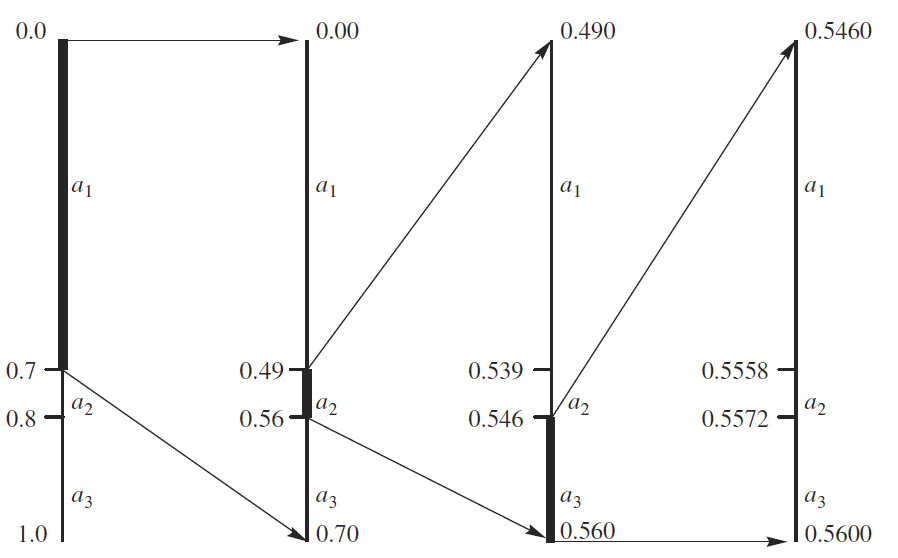
\includegraphics[width=0.6\textwidth]{figures/3_compression/arithmetic}
\caption{Arithmetic coding scheme in practice with the alphabet from Table \ref{tab:arithmetic} on the sequence $a_1,a_2,a_3$}
\label{fig:arithmetic}
\end{figure}

This kind of coding although easy to understand, it's actually quite cumbersome to directly implement on a computer, where only a certain floating point precision can be achieved. For real life use this precision is often unsatisfactory, so some extra steps are involved in the coding.

Since after each step the next subinterval is a subset of the previous interval, if the coding interval after a certain number of steps is contained in either the upper or lower half of the unit interval it will remain there for the rest of the coding. We can exploit this fact by rescaling that interval to the unit interval and writing either a 0 or 1 bit to the output depending on the position of the subinterval. By continuing this scheme it's possible to reach arbitrary precision even using a computer.

The decoding process is analogous to encoding. The decoder keeps track of the
current lower and upper bounds. It mimics the rescaling operations of the encoder
based on the bits of the encoded binary number.

\section{Transform coding}
The methods outlined in the previous section are effective at compressing the data in an optimal way and reaching the first order entropy, however the assume nothing about the structure of the data. For image compression it's important to also consider this, since most images have a relatively high level of autocorrelation, meaning that neighboring values have a high chance of being similar, although not necessarily equal. Transform coding is a technique that by itself does not compress the data, however by exploiting some knowledge of the structure it transforms the data effectively reducing it's first order entropy. When regular entropy coding is then preformed on the transformed data, because of the reduced first-order entropy, these techniques can achieve a higher rate of compression. At decompression, after decoding the entropy coder, the reverse transformation is applied to reveal the original data. In this section I will introduce two of the most important algorithms for transform coding, Discrete Cosine Transform and Wavelet Transform.
\subsection{Discrete Cosine Transform}
Discrete Cosine Transform \cite{ahmed_discrete_1974} is closely related to the well known Fourier transform. The main idea behind this is to represent a function by a weighted sum of different sine and cosine functions. This provides a different view, instead of looking at the data in the time domain, we gain information about the frequencies that compose the signal. 

Discrete Cosine Transform is a variant of the discrete Fourier transformation, however instead of making the signal periodic which can introduce large jumps at the edges, the signal is extended in a symmetric way. Since this will give a smooth transition even at the boundaries, the transform does not have to include so many high frequency components. Also, because of the symmetric extension, it's possible to represent the functions only by using the cosine bases, resulting in fewer coefficients. Overall, the DCT is much better suited for compression, than DFT.

The DCT base functions are defined in the following way:
\begin{equation}
c_{i,j} = s_i \cdot \cos \frac{(2j+1)i\pi}{2n} \qquad \text{with } s_i = 
    \begin{cases}
        \sqrt{\frac{1}{n}} & \text{if } i=0 \\
        \sqrt{\frac{2}{n}} & \text{otherwise}
    \end{cases}
\end{equation}
The scaling factors is are chosen so that the $L_2$ norm of each basis vector is 1 and
so the transform is orthonormal. The inverse transform can therefore be found by
simply transposing the transform matrix.

\begin{figure}
\centering
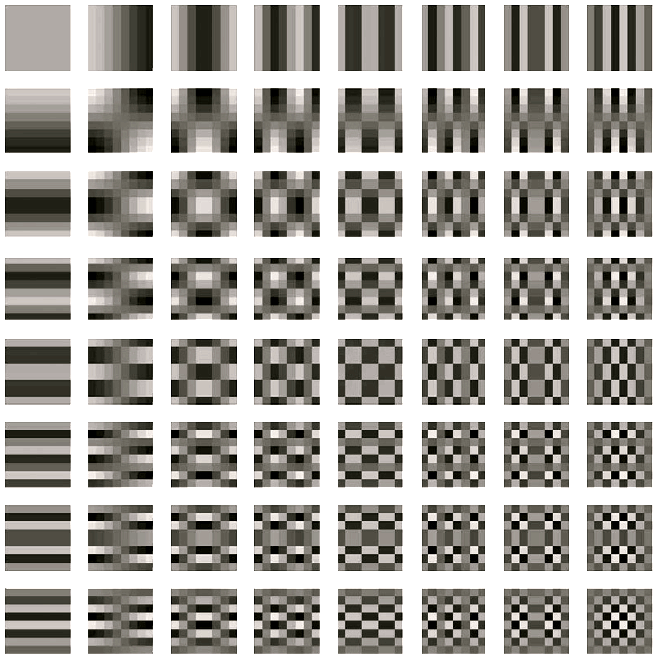
\includegraphics[width=0.4\textwidth]{figures/3_compression/DCT_bases}
\caption{Basis functions of the $8 \times 8$ 2D DCT, computed as the outer product of the 1D basis vectors.}
\label{fig:DCT_bases}
\end{figure}

Applying the DCT to two dimensional functions, i.e. images is very similar to the two dimensional Fourier transform. The base functions are the outer products oft the 1D base functions (Figure \ref{fig:DCT_bases}.), and the transform can actually be performed separately for each dimension.

Computation effort in a naive implementation is $O(n^2)$ but since DCT is based on the Fourier transform, an $O(n \log n)$ algorithm is also possible, analogous to the fast Fourier transform. This is still larger than a linear scaling with the data size, which can be very inconvenient. Therefore, in practice the DCT is usually applied to smaller blocks of the image, such as $4\times4$, $8\time8$ or $16\times16$. 

Although DCT is an effective way of reducing the first-order entropy, it has a potential shortcoming by its use of floating point arithmetic. Because of the finite machine precision inherent rounding errors will occur, which means the reverse transformation can not generate the exact original data. For many application, such as photography, this still can be acceptable, but for scientific image data lossy compression is generally not accepted.


\subsection{Discrete Wavelet Transform}
Methods based on Fourier analysis, such as the DCT introduced in the previous section, give excellent localization in frequency space: They tell us exactly which frequencies occur in the data, which is very useful for data compression. However, they give no spatial localization: They do not tell us where in the signal these frequencies occur. Every DCT base function affect the whole image domain, which means distinct local structures can have a global effect on the final outcome. In case of an edge for example, it's necessary to include a high frequency component with a large coefficient, but since every DCT base function has an impact on the whole domain, this will have to be compensated on smoother regions by also increasing the coefficients of other factors. This can negatively impact compression performance.

A solution for this is to use different base functions, namely ones with finite support. This way we will not only be able to get information about the frequency, but also about the localization of that frequency in some extent.

One option for such a set of local basis functions, and certainly the most popular one, is the multi-resolution analysis based on wavelets. The term “multi-resolution analysis” in the context of wavelets was introduced in the late 1980s by Stéphane Mallat \cite{mallat_theory_1989}, though research on wavelets had been ongoing for several years before that.

The idea behind the wavelet multi-resolution analysis is to build a basis out of translated and scaled versions of one underlying function called the \textit{mother wavelet} $\psi$. The mother wavelet is non-zero only in a small region, leading to the locality properties. It is translated to cover the whole domain. It also covers only a small frequency band, and is scaled to cover higher or lower frequencies. The family of translated and scaled functions $\psi_{l,i}$ is generated from   according to
\begin{equation}
\psi_{l,i}(t) = \sqrt{2^l} \psi \left(2^l t-i\right), \qquad l, i \in \mathbb{Z}
\end{equation}
Incrementing $l$ halves the width of the resulting function, which thus corresponds to a higher frequency band. Changing $i$ moves the function along the x axis. The size of each step scales with the width of the function, defined by $l$. The normalization factor $\sqrt{2^l}$ is chosen so that the $L_2$ norm stays constant. The mother wavelet can be chosen so that the $\psi_{l,i}$ are pairwise orthogonal and thus form a basis of some function space. However, representing a function in this basis will generally require an infinite number of basis functions $\psi_{l,i}$: To represent a constant component, i.e. content of frequency zero, the wavelet must be infinitely scaled. To address this, it is necessary to introduce an additional scaling function $\phi$ which complements the wavelet. It is scaled and translated the same way as the mother wavelet.

The oldest wavelets are the Haar wavelets, and because of their simplicity, they provide a good example on how wavelet transformation works. The Haar wavelet scaling $\phi$ and wavelet $\psi$ functions are the following:
\begin{equation}
\phi(t) = 
\begin{cases}
    1 & \text{if } 0 \leq t < 1 \\
    0 & \text{otherwise}
\end{cases}
\label{eq:scaling}
\end{equation}

\begin{equation}
\psi(t) = 
\begin{cases}
    -1 & \text{if } 0 \leq t < \frac{1}{2} \\
    1 & \text{if } \frac{1}{2} \leq t < 1 \\
    0 & \text{otherwise}
\end{cases}
\label{eq:wavelet}
\end{equation}
Clearly, all wavelet functions $\psi_{l,i}$ are orthogonal. Additionally, the scaling functions $\phi_{l,i}$ at a fixed level $i$ are orthogonal. The scaling functions $\phi_{l,i}$ are also orthogonal to the wavelet functions $\psi_{k,i}$, $k \geq l$ at the same and all finer levels.

Figure \ref{fig:wavelet}. (left) schematically shows the decomposition of a signal into low-pass components corresponding to the scaling function, and high-pass components corresponding to the wavelet. The signal $s_0$ can be represented by the translated scaling function at a finer scale $l_0$, which can be decomposed to the sum of a coarser approximation $s_1$ corresponding to the scaling function and the detail part $d_1$ corresponding to the wavelet functions. This decomposition to a sum of coarser approximation and detail can be continued multiple times, thus resulting in the previously mentioned multi-resolution analysis.


\begin{figure}
\centering
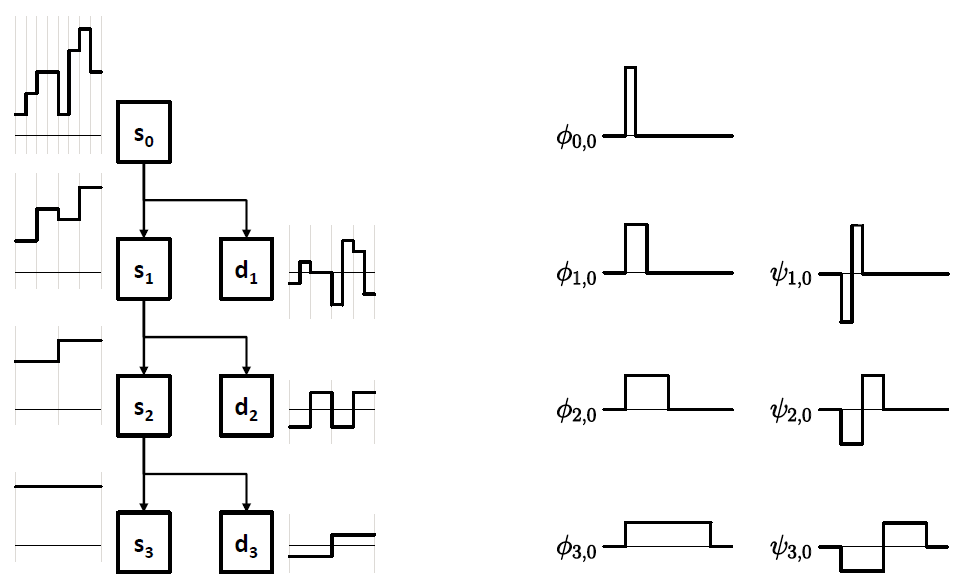
\includegraphics[width=0.6\textwidth]{figures/3_compression/wavelet}
\caption{Multi-resolution wavelet decomposition, using the Haar wavelets as an example. Left: decomposition to multiple levels of low pass and high pass coefficients corresponding to the scaling and the wavelet functions respectively. Right: some of the base wavelet functions used for the decomposition.}
\label{fig:wavelet}
\end{figure}


Of course, for image compression applications, it is desirable to extend this transformation to a 2D version, that can be applied to the images before performing the arithmetic coding. Similarly to the DCT, the wavelet transform is also separable, and can be performed as a sequence of 1D transforms along different directions. Separable in a sense, that it does not matter in which order the individual 1D DWTs are applied to get the same 2D transformation.

\subsection{Pixel prediction}



\section{Conclusion}
In this paper I have introduced some of the most important techniques for image compression. Many of these are used in different image compression algorithms, such as JPEG \cite{pennebaker_jpeg:_1992}, JPEG-LS \cite{weinberger_loco-i_2000} and JPEG2000. The common point for each of these formats is that they first transform the images to effectively reduce first order entropy, either by predicting the pixel values and coding only the differences (JPEG-LS), or by using either Discrete Cosine Transform (JPEG) or Discrete Wavelet Transform (JPEG2000). In the case of lossy standards after this transformation step a quantization is also performed depending on the desired quality setting for the coder. Finally as the last step the transformed and quantized coefficients are compressed by an arithmetic coder, such as Huffman coding in JPEG of arithmetic coding in JPEG2000. The end result in each case is a highly optimized compression that greatly reduces the file size.




\chapter{Real-time, GPU accelerated image processing pipeline}
\section{GPU architecture}

\section{Live fusion}
    \subsection{MuVi-SPIM}
    \subsection{Bead based registration}

\section{B³D image compression}
\b3d image compression
B³D image compression

\subsection{Data sizes in microscopy}

\begin{figure}[tpb]
 \centering
 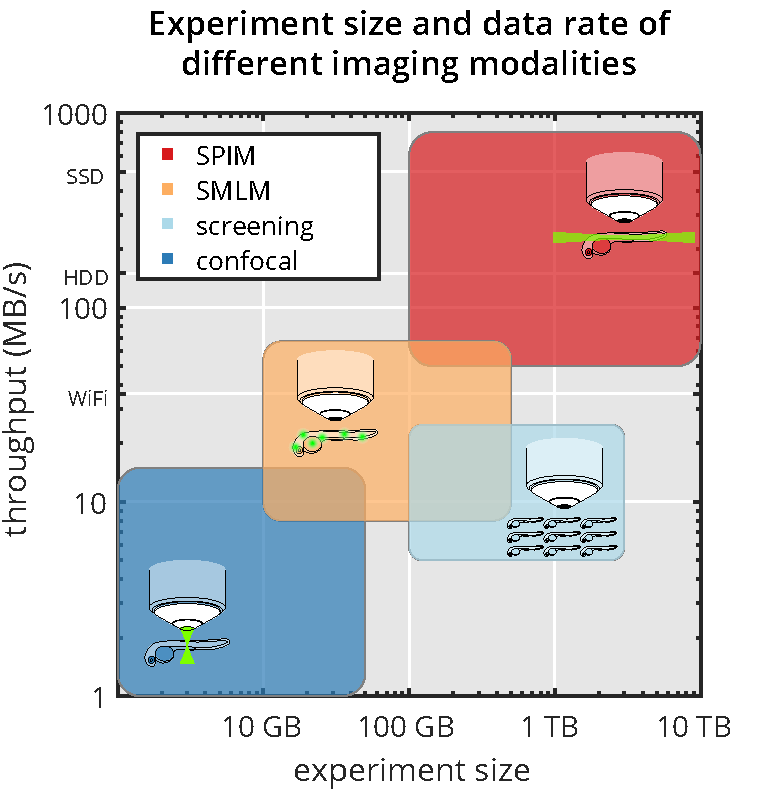
\includegraphics[page=1,width=0.6\textwidth]{figures/4_gpu/comparison_with_pictograms}
 \caption{\textbf{Experiment sizes and data rate of different imaging modalities.} Comparison of single-plane illumination microscopy (SPIM, red rectangle), high-content screening (light blue), single molecule localization microscopy (SMLM, orange) and confocal microscopy (blue) by typical experiment size and data production rate (see also Table \ref{tab:sizes}).}
 \label{fig:sizes}
\end{figure}


\begin{table}[tbp]
\begin{small}
\renewcommand{\arraystretch}{2}
\centering
\begin{tabular}{rp{5cm}cccc}
    & \textbf{imaging device} & \textbf{image size} &  \parbox[c]{1.2cm}{\textbf{frame}\\ \textbf{rate}} & \textbf{data rate} & \parbox[c]{1.2cm}{\textbf{data\\ size}} \\
    \hline
    \hline
    \textbf{SPIM} & 2x sCMOS camera (e.g. Hamamatsu ORCA Flash4.0) & 2048x2048 & 50/s & 800 MB/s & 10 TB \\ \hline
    \textbf{SMLM} & 2x EMCCD camera (e.g. Andor iXon Ultra 897) & 512x512 & 56/s & 56 MB/s & 500 GB \\ \hline
    \textbf{screening} & CCD camera (e.g. Hamamatsu ORCA-R2) & 1344x1024 & 8.5s/ & 22 MB/s & 5 TB \\ \hline
    \textbf{confocal} & Zeiss LSM 880, 10 channels & 512x512 & 5/s & 12.5 MB/s & 50 GB \\ 
\end{tabular}
\caption{\textbf{Data sizes in microscopy.} Typical devices used for confocal microscopy, high-content screening, single-molecule localization microscopy and light-sheet microscopy and their data production characteristics. Data visualized on Figure \ref{fig:sizes}}
\label{tab:sizes}
\end{small}
\end{table}

\subsection{Lossless compression performance}

\begin{figure}[tpb]
 \centering
 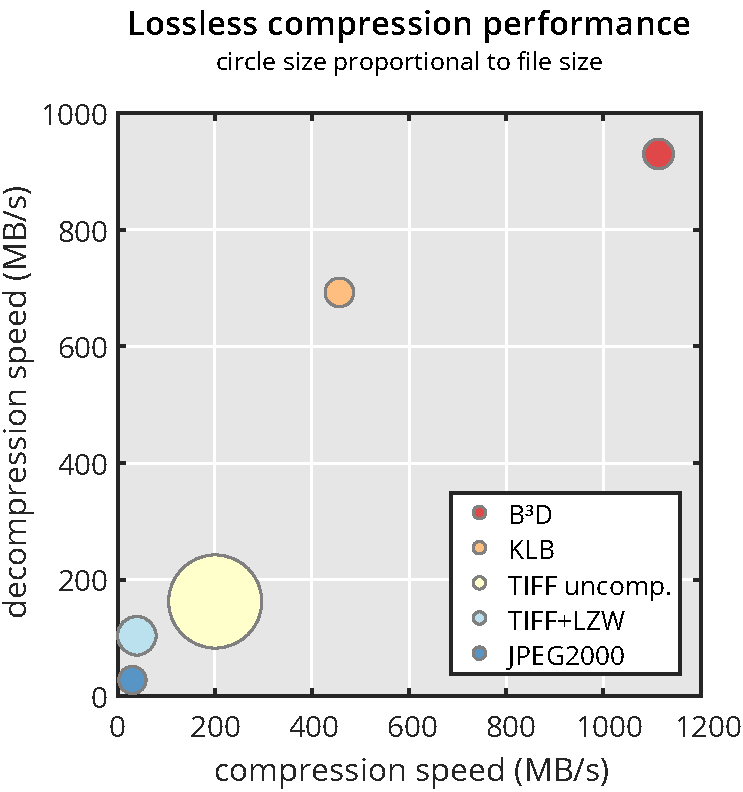
\includegraphics[page=1,width=0.6\textwidth]{figures/4_gpu/bubbles}
 \caption{\textbf{Lossless compression performance.} Performance comparison of our B³D \b3d compression algorithm (red circle) vs. KLB (orange), uncompressed TIFF (light yellow), LZW compressed TIFF (light blue) and JPEG2000 (blue) regarding write speed (horizontal axis), read speed (vertical axis) and file size (circle size). (see also Table \ref{tab:performance}).}
 \label{fig:performance}
\end{figure}

\begin{table}[tbp]
\renewcommand{\arraystretch}{2}
\setlength{\tabcolsep}{9pt}
\centering
\begin{tabular}{lrrrr}
    & \textbf{write speed} & \textbf{read speed} & \textbf{CR} & \textbf{file size} \\
    \hline
    \hline
    \textbf{\b3d} & 1,115.08 MB/s & 928.97 MB/s & 9.861 & 100\% \\ \hline
    \textbf{KLB} & 283.19 MB/s & 619.95 MB/s & 10.571 & 93.28\% \\ \hline
    \textbf{JPEG2000} & 31.94 MB/s & 26.38 MB/s & 11.782 & 83.69\% \\ \hline
    \textbf{JPEG2000} & 202.32 MB/s & 161.08 MB/s & 1.00 & 986.1\% \\ \hline
    \textbf{TIFF + LZW} & 40.85 MB/s & 102.37 MB/s & 5.822 & 169.37\%
\end{tabular}
\caption{\textbf{Lossless compression performance.} \b3d is compared with various popular lossless image compression methods regarding write speed, read speed and compression ratio (original size / compressed size). Data visualized on Figure \ref{fig:performance}.}
\label{tab:performance}
\end{table}

\subsection{Benchmarking}

\begin{figure}[tpb]
 \centering
 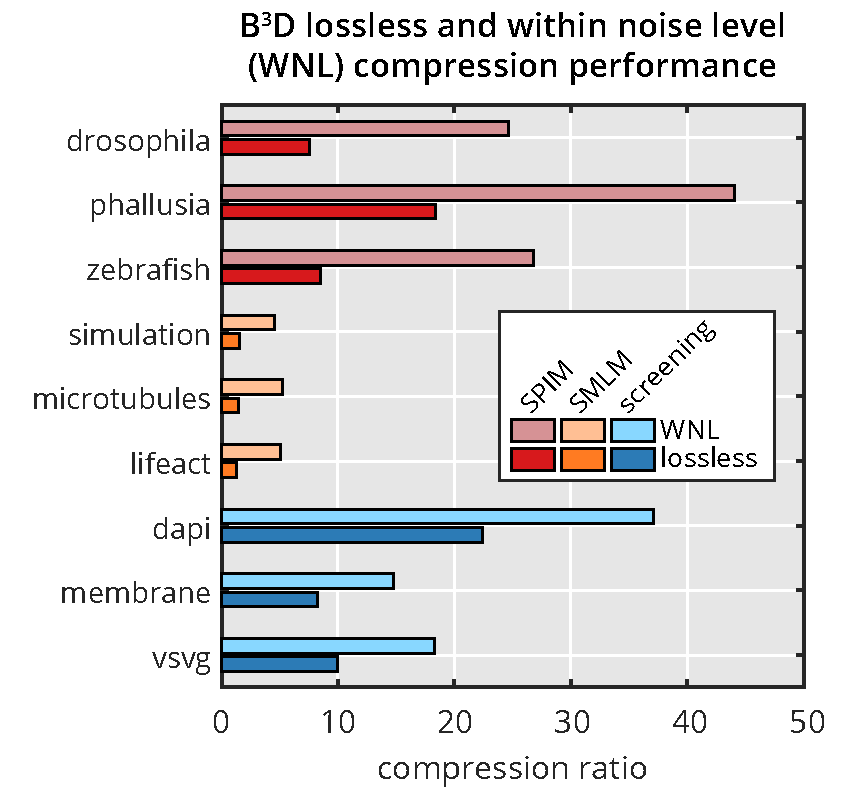
\includegraphics[page=1,width=0.6\textwidth]{figures/4_gpu/Fig1c_compressionBars}
 \caption{\textbf{Lossless compression performance.}  For description of datasets see Table \ref{tab:datasets}.}
 \label{fig:benchmark}
\end{figure}

\begin{table}[tbp]
\begin{small}
\renewcommand{\arraystretch}{2}C
\centering
\begin{tabular}{llp{7cm}r}
    \textbf{Dataset name} & \parbox[c]{2cm}{\textbf{Imaging\\modality}} & \textbf{Description} & \textbf{Size (MB)} \\
    \hline
    \hline
    \textbf{drosophila} & SPIM & dataset acquired in MuVi-SPIM of a Drosophila melanogaster embryo expressing H2Av-mCherry nuclear marker & 494.53 \\ \hline
    \textbf{zebrafish} & SPIM & dataset acquired in MuVi-SPIM of a zebrafish embryo expressing b-actin::GCaMP6f calcium sensor & 2,408.00 \\ \hline
    \textbf{phallusia} & SPIM & dataset acquired in MuVi-SPIM of a Phallusia mammillata embryo expressing PH-citrine membrane marker & 1,323.88  \\ \hline
    \textbf{simulation} & SMLM & MT0.N1.LD-2D simulated dataset of microtubules labeled with Alexa Fluor 647 from SMLMS 2016 challenge & 156.22 \\ \hline
    \textbf{microtubules} & SMLM & microtubules immuno-labeled with Alexa Fluor 674-bound antibodies in U2OS cells & 1,643.86  \\ \hline
    \textbf{lifeact} & SMLM & actin network labeled with LifeAct-tdEOS in U2OS cells & 3,316.15  \\ \hline
    \textbf{dapi} & screening & wide field fluorescence images of DAPI stained HeLa Kyoto cells \cite{simpson_genome-wide_2012} & 1,005.38 \\ \hline
    \textbf{vsvg} & screening & wide field fluorescence images of CFP-tsO45G proteins in HeLa Kyoto cells \cite{simpson_genome-wide_2012} & 1,005.38  \\ \hline
    \textbf{membrane} & screening & wide field fluorescence images of membrane localized CFP-tsO45G proteins labeled with AlexaFluor647 in HeLa Kyoto cells \cite{simpson_genome-wide_2012} & 1,005.38  \\ 
\end{tabular}
\caption{\textbf{Datasets used for benchmarking compression performance.}}.
\label{tab:datasets}
\end{small}
\end{table}

\section{Noise dependent lossy compression}

\section{Methods}


\chapter{Discussion}

\newpage
\cleardoublepage
\phantomsection
\begin{acknowledgements}

I would like to thank Lars Hufnagel for this opportunity to work in his group, and involving me in developing this microscope system. He gave me a lot of support, and helped in understanding and solving the possible difficulties that we came across during the development process.

I greatly appreciate the help of Uroš Kržič, who gave me an insight on the principles of selective plane illumination microscopy, and also prepared some illustrations for this work.

I thank Stefan Günther for providing the \textit{Drosophila m.} embryos, and \mbox{Ulla-Maj} Fiuza for providing the \textit{Phallusia m.} embryos.

Finally, I would like to thank Gustavo Quintas Glasner de Medeiros and Nils Norlin, as they both participated in the microscope design and program development, and both of them inspired me greatly. Without their help, I couldn't have written this paper.

\addcontentsline{toc}{chapter}{Acknowledgements}
\end{acknowledgements}

\cleardoublepage
\phantomsection
\addcontentsline{toc}{chapter}{References}
\bibliographystyle{IEEE/IEEEtran}
{ \small \bibliography{EMBL}}


\end{document}
